%  
% Features:
%  � Proper page sizes as required by university guide for students:
%      � proper font sizes as well as linespacings
%      � proper size of margins
%  � Generic title page:
%      � \gentitle
%  � Generic abstract page(s):
%      � \begin{itabstract}{Keywords}
%          abstract text
%        \end{itabstract}
%      � \begin{ittiivis}...\end{ittiivis} provides finnish version
%         � ittiivis defaults to finnish so no need to issue 
%           \selectlanguage{finnish}
%      � total number of pages as well as total number of pages in appendices
%        are automagically handled
%  � Entry environment:
%      � \begin{entry}[widest label]
%          \item[1st label text] ...
%          \item[2nd label text] ...
%        \end{entry}
%      � the actual items are aligned to suit the widest label, which is
%        given as an argument to the environment
%  � Use of specific latex packages to ease in formatting the thesis:
%      � format table of contents to have bibliography shown as references
%        as well as other fixes           (tocbibind)
%      � enhanced verbatim handling       (sverb)
%      � source code inclusion            (listings)
%      � handling of headers and footers  (fancyhdr)
%
%      � consultation of the manuals of these packages is strongly
%        encouraged 
%
% Assumptions:
%  � itpackage.sty file is available 
%  � each chapter is as a separate file which is read in with e.g. \input
%   
% Miscellaneous:
%  � comments are welcome
%  � should a required package be missing see http://www.ctan.org/ 
%  � http://www.ctan.org/tex-archive/info/lshort/english/lshort.pdf
%
%%%%%%%%%%%%%%%%%%%%%%%%%%%%%%%%%%%%%%%%%%%%%%%%%%%%%%%%%%%%%%%%%%%%%%%%%%%

\documentclass[a4paper,12pt]{report}
% ams-packages for maths
\usepackage{amssymb,amsthm,amsmath}

% babel-package for automatic hyphenation
\usepackage[english,finnish]{babel}
\usepackage[latin1]{inputenc}

% load graphicx package
%   � automagically select proper parameters depending on whether
%     we're running pdflatex or latex
%   � specify \includegraphics{file} without the file extension
%     (.eps /.pdf (/ .png / .jpeg / ...)), tex should select the proper file
%
\usepackage{ifpdf}
\usepackage{graphicx}

% load tocbibind package 
%   do not include table of contents in itself
%   convert the name of bibliography to references
\usepackage[nottoc]{tocbibind}
\settocbibname{References}

% load sverb package
% enhanced handling of verbatim stuff; listing environment
\usepackage{sverb}
\usepackage{acronym}

% load listings package
% handle inclusion of source code
\usepackage{listings}
\usepackage{color}
\usepackage{url}

% load fancyheaders package
% the actual headers and footers are set later
\usepackage{fancyhdr}

% load itpackage 
% additional defines and stuff
\usepackage{itpackage}
\usepackage{float}
\floatstyle{boxed} 
\restylefloat{figure}

\graphicspath{{./img/}}

\renewcommand{\topfraction}{.85}
\renewcommand{\bottomfraction}{.7}
\renewcommand{\textfraction}{.15}
\renewcommand{\floatpagefraction}{.66}
\renewcommand{\dbltopfraction}{.66}
\renewcommand{\dblfloatpagefraction}{.66}

\setcounter{topnumber}{9}
\setcounter{bottomnumber}{9}
\setcounter{totalnumber}{20}
\setcounter{dbltopnumber}{9}

% main document starts here

\definecolor{dkgreen}{rgb}{0,0.6,0}
\definecolor{gray}{rgb}{0.5,0.5,0.5}
\definecolor{mauve}{rgb}{0.58,0,0.82}

\lstset{frame=tb,
  language=Java,
  aboveskip=3mm,
  belowskip=3mm,
  showstringspaces=false,
  columns=flexible,
  basicstyle={\small\ttfamily},
  numbers=none,
  numberstyle=\tiny\color{gray},
  keywordstyle=\color{blue},
  commentstyle=\color{dkgreen},
  stringstyle=\color{mauve},
  breaklines=true,
  breakatwhitespace=true
  tabsize=3
}

% Hyphenation within texttt
\DeclareFontFamily{\encodingdefault}{\ttdefault}{\hyphenchar\font=`\-}

\begin{document}
\lstset{language=Java}

%%% fill in your information below
\workinfo
{Oma Nimi}
{Manolia CMS. Next Generation CMS Development With Vaadin |OR|
 Magnolia CMS and Vaadin. Integration of an Application Framework in CMS Development Process.
  
}
{Tarkastaja yksi}
{Tarkastaja kaksi}
{Vuosiluku}
{Month}
{Kuukausi}
%% set the type of your thesis (Diplomity�, TkK -tutkielma, etc.) below
\worktype{Type of  thesis}{Ty�n tyyppi}
 
%% set the laboratory or field of study
\deptinfo{Laboratory Name}{Labran Nimi}

% generate the title page 
\gentitle
% generate abstract
\begin{itabstract}{list, of, keywords}
Here comes a short abstract.
\end{itabstract}

% select language here (note that english also needs to set enclname)
%\selectlanguage{finnish}
\selectlanguage{english}\def\enclname{Appendices}

% empty pagestyle for table of contents etc. 
%
% the redefinition of plain style works also for 1st pages of chapters,
% which is the default in report class. Just state \thispagestyle{empty}
% after \chapter{something} if you want empty style for the 1st pages. 
%
\pagestyle{empty}
\fancypagestyle{plain}{
  \fancyhf{}
  \renewcommand{\headrulewidth}{0 pt}
}

% roman numbering for table of contents etc.
\pagenumbering{roman}

% insert table of contents, list of figures, list of tables
%
% setting the counter to zero effectively removes the page number from
% the toc, lof etc. entries in the toc since there is no roman numeral
% for zero ;-) (if you want them without numbering)
%
%\setcounter{page}{0}

%********************************%
%Table of Contents               %
%********************************%
\tableofcontents
\clearpage

\setcounter{page}{0}
%********************************%
%List of figures                 %
%********************************%
\listoffigures 
\clearpage
\setcounter{page}{0}

%********************************%
%List of tables                  %
%********************************%
%\listoftables

% possibly insert 'list of acronyms'
%
%   create a chapter called List Of Acronyms (or whatever), which
%     should contain all your acronym definitions, e.g. 
%     \chapter{List Of Acronyms} 
%   the secnumdepth trickery is needed because acronyms are as a
%     standard chapter and we are faking '\listofacronyms'
%
%\setcounter{secnumdepth}{-1}
%\input{your acronym chapter's file name}
\setcounter{secnumdepth}{2}
% setup page numbering, page counter, etc.
\startpages
\lstset{language=Java}
\setcounter{chapter}{0}
%\chapter{Introduction}

World Wide Web (www) plays a significant role in all aspects of our life. It is
a great source of information, key point in business and an easy way for
communication. The building blocks of the WWW are the websites. But what does it
take to make a feature rich, efficient website that is optimized for web search?
Several ways are possible. One obvious option would be to hire a team including
the experienced web-developers, designers and Search Engine Optimization (SEO)
experts. This approach usually allows to achieve the desired result with low
amount of risk. However, the price and development time could also be very high.

The other option is to use a Content Management System (CMS). CMS is a program
or a set of programs used for building websites. Normally CMS is controlled
through some kind of user interface that allows to handle most of the typical
yet crucial tasks out of the box. The main functions of almost every CMS is the
association of content and data with some kind of a rendering mechanism. As a
result the project team can concentrate mostly on business logic and the actual
content while it's presentation can be successfully covered by, for instance, a
CMS template kit. Other tasks that CMS can handle include storing and sharing
data between users, access and user role management, Web pages design,
deployment etc. There are CMS's that could be a great foundation for almost any
fundamental type of web project in various areas like e-commerce, blogs or
social networks. In some cases CMS could let the developer complete the project
without any developer or designer skills.

The biggest problems that could be experienced while using a CMS are usually
related to either steep learning curve or to limitations of the administration
tools. It is especially common in the area of enterprise-oriented Content
Management Systems. The vendor of a powerful CMS has to find a balance between
clear, convenient and intuitive UI and the richness of the functionality in
order to provide customers with full control over their websites. It is also
important that the administration program supports customization.

Magnolia CMS is one of the leading open source Content Management Systems. The
main focus of Magnolia is medium to large enterprise projects. Magnolia CMS is
written in the Java programming language and incorporates various best of breed
Java technologies: data management implemented on top of Jackrabbit (Java
Content Repository implementation), core Application Programming Interface (API)
architecture based on Google Guice dependency injection framework, distribution
and building is handled by Apache Maven.

AdminCentral is one of the most important Magnolia modules. It is the
administration tool of the CMS. The module allows to manipulate the data in JCR
repositories, to run queries and to edit pages with a visual page editor.
The thesis under consideration describes the development of the fifth generation
of Magnolia CMS. The most significant innovation of the new CMS version is the
AdminCentral module developed on top of the Vaadin framework. The main target of
the project is to make the process of administration highly flexible,
customizable and simple.

The cornerstone concept of Magnolia 5.0 is the modular structure based on the
application metaphor. It provides a clear and intuitive understanding of the
system administration principles. This concept also allows the customers and
community contributors to build their own application modules based on simple
API's and to integrate those into the Magnolia admin interface with almost no
effort.

The first chapter of the current text is devoted to the more detailed CMS world
overview. The definition and goals of CMS's will be stated. We will examine the
main types of the existing Content Management Systems, their common useful
features and typical pitfalls. A special emphasis will be devoted to the
position of the Magnolia CMS.

In the following chapter summarizes the main problems that the project under
consideration (Magnolia 5.0) tries to solve. For instance, we will study why it
is improtant that a CMS has a decent support for mobile platforms, what it takes
to create such CMS that is extensive and convenient for user.

Then we will proceed to the observation of the technology stack used in the
considered project (Chapter 4). Even though the range of the used libraries,
frameworks and API's is quite vast - we will examine the most important of them.
For example, the main features of Vaadin, GWT, JQuery and Magnolia CMS itself
will be discussed.

In chapters 5 and 6 we will concentrate on the project's architecture and
implementation. The high-level architecture outlines will be provided in the
chapter 5: the used frameworks role distribution and the relations between them.
The main patterns and concepts of the system that play the most significant
roles will be studied separately. Additional attention for instance will be
devoted the application framework which is the crux or of the project's
architecture.

In chapter 6 we will focus on the implementation details. In that scope we will
study the data binding between Magnolia CMS and the Vaadin framework, some
client-side peculiarities and a sample application development with Magnolia CMS
API.

Finally, we will discuss the the potential flaws and possibilities for the
project's improvement especially by means of the latest version the Vaadin
framework.

Key words: Magnolia CMS, Vaadin, GWT, JQuery, J2EE.
\pagebreak

%\chapter{CMS}
Before we start analyzing the strcture and the implementation details of a new
generation CMS it is worth giving a definition to a Content Management System.
Apart form that in the current chapter we will discuss the types of CMS's that
exist nowadays. Finally, we will concentrate on the Magnolia CMS which is the
target system of the current paper: the high-level structure and main features
of it will be highlighted.

\section{Definition of a CMS}
A \emph{Content Management System or CMS} could be defined as a server-side
software that is designed to simplify the creation and maintenance of websites.
These systems manage online content, generate Web pages, and allow users to
upload and change content without requiring technical expertise. The foundation
of almost every CMS is a data storage of a varying type like, for instance, a
database or a repository which stores the content allowing it to be reused,
repurposed or published on demand.

Another crucial part of every CMS is the administration interface. It interacts
with the storage and provides users with various tools starting from
input/upload of content to complex editors and asset managers.
Typically this administration interface is implemented in the form of a web
application. The biggest advantage of this approach is that the actual content
resides within easy reach from any location having internet access.

However, acting just as a data storage management tool would not make any CMS a
valuable or highly useful product. The main purpose of a CMS is to build the Web
Site around the content. This involves several fundamental concepts:
\begin{itemize}
	\item Template mechanism. Normally the system is shipped with the  templating
	framework. This framework is a higher level abstraction on top the ordinary
	programming language and allows for the building of complex pages with less
	effort.
	Applying the specific template to the raw content from the repository is a
	concept idea of making web-pages with CMS's.
	Different systems offer different levels of flexibility allowing to partially or
	completely change the templates, or to create new templates and themes.

	\item Automation of page generation. A CMS often provides the engine that would
	generate the typical pages on demand or request. A good example would be a blog
	post or a forum thread.
	
    \item Navigation handling. A CMS provides an easy and almost automated way to
    set references between parts of the web site and to manage them on the high
    level.
	
	\item Basic Search Engine Optimiation (SEO). (TODO: Add how)
\end{itemize}


\section{Types of CMS} 
There are numerous CMS's existing nowadays. As it was mentioned
before a CMS can be developed with different programming languages, e.g.
\emph{Plone CMS} is written in Python, \emph{Drupal} and \emph{Joomla} are
written in PHP and \emph{OpenCMS} is written in Java \cite{cms_list}.

Each CMS is trying to occupy some certain niche and to solve problems of
different scope. There are some systems that are highly powerful only for some
specific use cases, for instance \emph{Wordpress} is primarilly used for developing
blogs \cite{wordpress} and \emph{Liferay} is a platform for the portals \cite{liferay}.

There are both proprietary (like \emph{Alphresco}) and open source CMS's (like \emph{MODx}).
The licences and usage policies also vary \cite{cms_list}.

\section{Importance of CMS's in the Modern World Wide Web}
Content Management Systems play a significant role in modern web development.
There are several strong reasons for that.

First of all, as it was mentioned before, adopting a CMS in the project provides
a solution for the most common problems a website developer faces. This can
dramatically increase the development speed allowing the team to concentrate on
business logic and higher level problems. In addition if the project is built on
top of a popular CMS - the chances of finding a relevant expert are a lot higher
than in the case of a completely custom made project.

What is more, a CMS offers a solid foundation which makes it easier to build
scalable, robust and responsive websites: many CMS's provide architecture for
clustering, while a time proven storage API ensures the safety of the data.

Another important advantage of Content Management Systems is that people without
advanced technical skills can use them.
A CMS with a powerful administration interface usually does not require
programming experience (neither client side like JavaScript/HTML/CSS, nor server
side like PHP or Java) to edit or add a page, upload data or change user
permissions. As a consequence the support of CMS-based projects is a lot
simpler. After shipping the product the development team can usually educate the
customer on how to use the admin tool and at least partially delegate the
maintenance chores to them.

There is no surprise in that almost one third of all websites in the WWW use a
CMS. The tendency depicted in Figure 1 shows that this amount is growing
\cite{cms_growth}.
\begin{figure}[H]
	\centering
	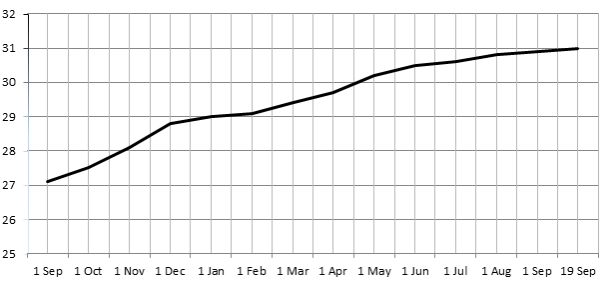
\includegraphics[width=\textwidth]{cms_usage_growth.png}
	\caption{CMS usage growth trend}
	\label{fig:cms_usage_growth}
\end{figure}

\section{Drawbacks of Using a CMS}
Obviously a CMS is not a silver bullet for all the problems. In spite of
reducing the project costs, speeding up the development process and allowing
users to avoid any kind of programming, usage of a CMS has several negative
aspects that should be kept in mind.

Sometimes non-technical companies adopt a CMS only in order to avoid learning
any programming language. This might not prove itself on the long run because
sooner or later a certain level of programming proficiency will be required.
This is dictated by the limitations of the templating mechanism which usually
requie designer skills to be properly surpassed.

Another case is the limitations of the administration interface: the specific
projects' authors might for example requires a special search tool or they need
to be able to observe the structure of their website in a form that is different
from those offered by the CMS they use. Finding a workaround would require some
backend programming experience or outsourced professional's help.
The complexity of the solution also depends a lot on the CMS administration
tools' ability to be extended. A good proof of such drawback could be the
results of the survey conducted by the Webcredible company several years ago.
According to it the practical factors such as the range of the offered features
(22 per cent), convenience (21 per cent) and ability to customize the
functionality were key when choosing a CMS. According to the Webcredible
authorities the results showed a high amount of respondents who were frustrated
with the poor user experience with the chosen CMS. The main reason for
dissatisfaction was the lack of attention to the end user needs resulting into a
product that is oriented on the technical people. Inability to extend the
system, add and replace modules on demand was also mentioned as a reason against
some systems \cite{poor_cms_experience}.

\section{Magnolia CMS}
The Magnolia CMS is one of the leading enterprise-oriented CMS's. It is
implemented using the Java programming language by Magnolia ltd., a company
located in the city of Basel, Switzerland. Magnolia is based on Jackrabbit
(JSR-170/JCR reference implementation) and focuses on medium to large
enterprises \cite{magnolia_cms_website}.

\subsection{Features of Magnolia CMS}
As long as Magnolia CMS is the main subject of this paper let us observe the
main features and advantages of the system, the position that it holds in the CMS world.

\subsubsection{Modular Structure}
The architecture of Magnolia CMS can be described as loosely coupled and
flexible. The system consists entirely out of modules.  A module is an
independent component that performs a particular task or packages content and
functionality \cite{book_of_magnolia}.
A good module example could be the AdminCentral (an admin interface of the CMS)
or the Blossom (Spring Framework Integration Module). A module can be used to
encapsulate a specific solution or a feature implementation e.g. a forum module
which is used for building discussion threads. It is also possible to make asset
bundles that can contain images or documents.
In some cases it becomes convenient to package an entire website with all the
content and templates to for example increase the deployment speed.

\subsubsection{Templating}
All Web pages created with the Magnolia CMS are based on templates. Templates
ensure that page structure and presentation remain the same while the content
varies from one page to another. For example, an event template helps you
generate event pages that look and feel the same while each of them displays a
different unique event.

The system generates pages by merging a template with corresponding content from
the repository. The position and inclusion of each paragraph on the page is
defined by the page template. In many instances, the page template will allow
authors to choose from a number of different paragraph types in a single content
area \cite{book_of_magnolia}.

\subsubsection{Scalability}

The Magnolia CMS is distributed as two web-applications, one acting as the
authoring instance and the other as the public environment (see \ref{fig:scalability}). This allows for
better security, having one application inside your firewall and one outside. It
also enables clustering configurations.
\begin{itemize}
	\item Author instance is where all authors work. It typically resides in a
	secure location such as behind a corporate firewall, inaccessible from the
	Internet. The author instance publishes content to public instances.
	\item Public instance receives the public content and exposes it to visitors on
	the Web. It resides in a public, reachable location. It is possible to have more
	than one public instance serving the same or different content.
\end{itemize}
\begin{figure}[H]
	\centering
	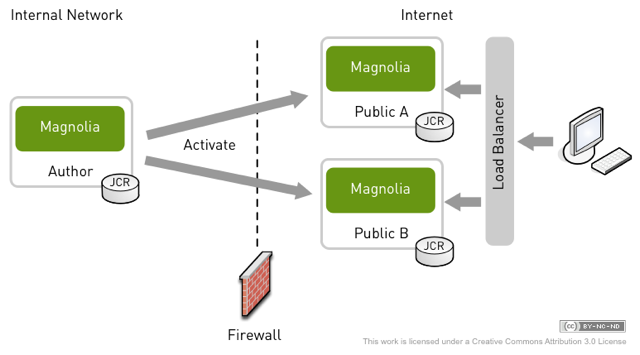
\includegraphics[width=\textwidth]{scalability.png}
	\caption{Magnolia CMS scaling strategy}
	\label{fig:scalability}
\end{figure}

\subsubsection{JSR-170}
Java Content Repository (JCR) is the core underlying technology for storing and
managing data in Magnolia CMS. JCR is a standard programming interface for
communication with content repositories. JCR was first established in Java
Specification Request 170 (JSR-170). Current JCR version 2.0 was finalized in
JSR-283. JCR is able to handle both structured and unstructured content
specified within hierarchical storage. Magnolia CMS uses Apache Jackrabbit
reference implementation of JCR and within the scope of current paper adheres to
the Java Content Repository standard.

\paragraph{Content Repository} stands for a high-level data management system
allowing for various operations to be performed over the stored content. These
are the most essential features of a Content Repository:

\begin{itemize}
  \item Aforementioned ability to store either structured content (e.g. Extensible Mark-up Language (XML)
  files, page templates etc) or unstructured (e.g. Binary Large OBjects (BLOB)).
  \item Referential integrity: support for primary and foreign keys and handling
  the violation of them.
  \item Querying data. The typical language to acces content repository is XML Path Language (XPath) \cite{xpath} 
  XPath. However, Structured Query Language (SQL) dialects usually can also be used.
\end{itemize}

A Magnolia CMS instance works with a single repository (called
\texttt{magnolia}). Semantic separation between datasets is provided with
\emph{workspaces}. Workspace is a tree-like structures with a single root.
The leaves of such a tree are called \emph{properties}. \emph{Properties} carry the all the
actual content of the repository.

From the perspective of this thesis, the most important workspaces of the Magnolia CMS are:
\begin{itemize}
  \item \emph{website} Stores the pages, paragraphs and most of the content  for the websites.
  \item \emph{config} The configuration settings.
  \item \emph{DAM} Workspace for Dynamic Asset Management.
  \item \emph{users} Stores all the types of user accounts (administrative, system public etc).
\end{itemize}

 We will especially concentrate on the \emph{config} workspace as configuration
 will play a significant role in the
foundation for the flexible user interface (see Chapter \ref{architecture}). We will
also touch the \emph{DAM workspace} when we will discuss the Asset Management in
the Chapter \ref{implementation}.


\subsubsection{Admin Central}
The Admin Central is the core module of Magnolia which gives the chrome for
administration and website management. Provides tools for editing publishing
and verifying the pages.\cite{magnolia_shell}

\subsubsection{Position in the CMS World}
Due to a flexible and highly customizable architecture that follows the best
Java patterns and practices, Magnolia CMS has managed to attract many serious
enterprises. Such companies as Allianz, Foxtel, Sony, Thomas Cook, Michelin,
U.S. Navy, Rewe, MBC Group, EADS, ING Bank, Atlassian and Migros and many others
in more than 100 countries \cite{magnolia_customers}.
\pagebreak
%\chapter{Targets for Magnolia 5.0}
\label{thesis_problems}

In previous chapter we have made an overview of the CMS world and introduced
Magnolia CMS and its strong sides and advantages. This chapter will be devoted
to the drawbacks and possibilities for the improvements of Magnolia. The main aspects we
are going to discuss will be the user experience and structural issues.

\section{Current Status of the System}
The latest release of CMS was Magnolia 4.5. The most crucial improvement it had
was the enhancement of the core API's and low-level functionality. The release
included the reworked Standard Templating Kit, upgrade of the Dependency
injection to be based on Google Guice. This release concentrated on the backend
improvements, pending system updates and refactorings in order to clear the way
for the different major enhancement of CMS - the user experience. Thus, the main
emphasis in this paper will be put on the Admin Central improvements for
Magnolia CMS 5.0.

The importance of a CMS admin interface was discussed before. It needs to have
an intuitive yet powerful user interface (UI) that provides great user
experience. [TODO: rephrase this.]It plays maybe the most significant role in
persuading the developers to use considered CMS. On the other hand, even
incredibly powerful CMS with poor user interface could make it next to unusable.

The current stable Magnolia CMS AdminCentral is based on the homegrown
JavaScript library (see \ref{fig:old_admin_central}). Even though it has gained
quite positive feedback due to it's minimalistic and clear design it is already
clear that it needs major improvements.

The main problem with the current Magnolia CMS AdminCentral module is related to
its structure which is not adapted for extensive changes and improvements. With
new versions new features are introduced that require various visual controls to
be added to the AdminCentral interface. However, it turned out that just
inflating the existing concept wouldn't work.
Users who tested and reviewed the first attempts of interface enhancements
weren't satisfied with the usability anymore.
Mainly they missed Magnolia's ease-of-use and lightness of appearance
\cite{bkg_of_new_design}.

A similar demand is heard from the community. The JavaScript (JS) library is not
a framework by design, indicating that a new component would require major
changes making it very hard for the third party developers to break in with
their code.
Thus even though over 70 additional modules exist for Magnolia, the development
and maintenance of those is a quite tedious task sometimes and far from all the
ideas can be implemented.

In order to solve the problem it would be quite logical to come up with an admin
module that acts not only as a user interface but also as a the framework which
has a modern solid look and feel while providing the clear and easy way to
extend itself.

As Boris Craft said in his interview to Dr. Dobbs: \emph{"Although the content
management system is typically seen as a website development tool, Magnolia is
seeking to provide the core services of the CMS proposition as a set of tools
for developers faced with bringing an increasing number of backend application
elements to the Web. This action, essentially, represents a decoupling of the
traditional elements of a CMS"} \cite{drdobbs_cms_decouple}.
\begin{figure}[H]
\begin{center}
  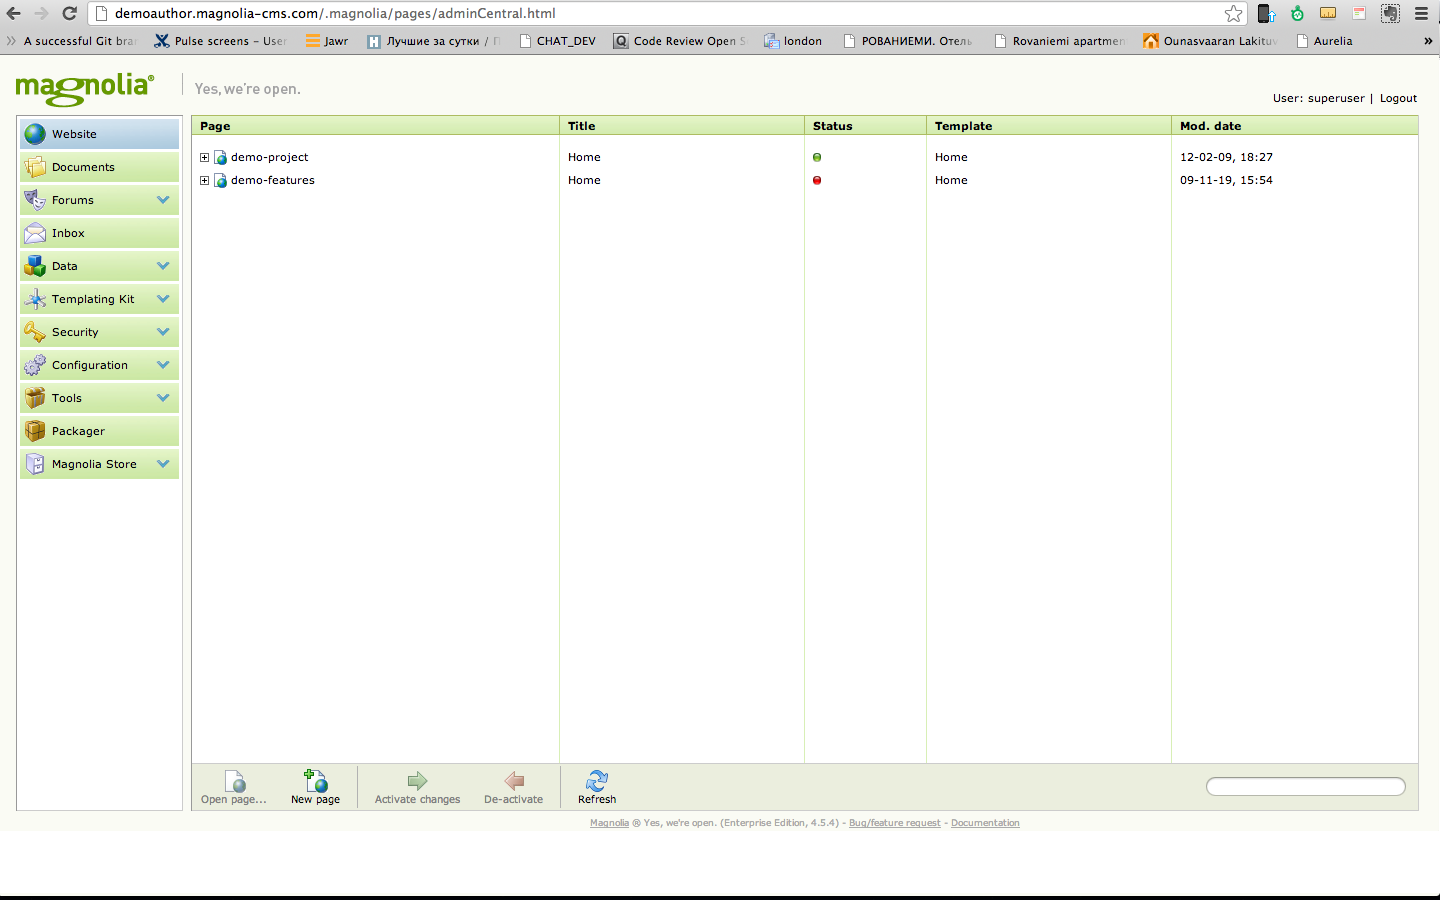
\includegraphics[width=\textwidth]{old_interface_magnolia.png}
  \caption[labelInTOC]{AdminCentral of Magnolia CMS 4.5}
  \label{fig: old_admin_central}
\end{center}
\end{figure}
However, this task is rather abstract and probably needs elaboration. Let us
observe the more specific assignments that could be spawned from it.

\section{Decoupling the Functionality of the Admin Interface}
Under decoupling here we mean separating the parts of interface into the logical
pieces that would describe themselves well and allow for adding the new ones
easilly. In order to provide the decoupling of current monolitic AdminCentral
interface there should be well-defined functionality units within the module.
Such units should cover a clear subset of the Magnolia CMS features just like an
application from the software suite. Thus, it makes sense to call the distinct
parts of a new interface \emph{applications} or simply \emph{apps}.

Developing the internal application framework is the key task in achieving the
final goal. The applications must be easy to build, integrate and style. In
spite of the distinct purposes and looks apps must have a common design.
Building an app should also require the least amount of boilerplate code. This
implies that a set of initial reusable components should be carefully designed
in order to reduce the boilerplate in the application code. It is also important
to develop the communication mechanism so that it is easy to send messages
between the apps.

\section{Improve Development Simplicity}
One of the biggest complexities in modern web application development is the
demand of mastering several programming languages and paradigms in order to
complete almost any project. Magnolia 5.0 targets reducing the amount of
technologies the app developer has to be familiar with (average knowledge of the
Java programming language should be enough). The client-server communication
should also be simplified as much as possible. As a consequence it would mean
abandoning the current Javascript based UI solution of AdminCentral and bringing
as much of its logic to server side as possible.
We will study how the task of building fully functioning web components can be
done without the involvement of client side programming by means of the Vaadin
application framework.

\section{Mobile First}
Mobile device platforms are becoming more and more popular nowadays. This is
mainly due to overcoming the technical barriers. The latest advancements in
technology progress gave users the hi-speed mobile Internet connection (3G, LTE)
the smartphones and tablets with computation power comparable to desktops. This
provides people with an opportunity to do the same tasks and jobs on mobile
devices as on the desktop computers. As a result - half of the world's web
traffic is mobile \cite{virtual_presence}.

There is a new trend called BYOD (Bring Your Own Device) - a movement or a
tendency of employees to use their own hardware at work. It has its roots in bad
user experience: people bring their devices to work because they want to
recreate the ease of use that they experience at home \cite{bkg_of_new_design}.
The main concept of BYOD is the requirement that the used software functions as
good on all major platforms and ideally - identically. Also it is hard to argue
with Borise's Kraft saying:
\emph{'If you compare today's bloated interfaces of enterprise software with the
fun-to-use, task-oriented apps on your iPhone you will immediately realize the
attraction of the latter'} \cite{mobile_first}.

Thus, supporting at least the major players in the mobile market (e.g. Apple iOs and
Google Android) is a must for Magnolia 5.0. This would involve the recognition
and support for touch events and gestures in order to give the editors the same
power as by the desktop version. 

\section{Performance and Scalability.}
The new interface must be scalable in terms of performance - visualization of
the tree structures with thousands of nodes must not be a problem. Data
management must avoid loading and keeping large datasets in memory and instead
rely onto lazy loading and caching mechanisms. For security reasons, the least
attainable amount of business logic should be exposed on the client side. 

UI scalability is also a requirement - in order to support extensions essential
Admin Interface has to support modular plugins a lot like modern mobile platforms 
support additional applications to be installed.

\section{CMS Deconstrution.}
The importance of a CMS admin interface was discussed before. It plays one of the
most significant roles in persuading the developers to use considered CMS. On the
other hand, even incredibly powerful CMS with poor user interface could make it
next to unusable.

Never the less, there is an indirect reason for struggling for delivering good
user experience. This reason is a lowering price and complexity of the other
systems' parts. The reduction is achieved by adopting the third-party products.
Indeed more and more utilities provided by a management suite can be separated
from it and be available as services. It is a common case that these sevices are
remote and even free. For instance, it makes little sense to develop the video
publishing and hosting facilities within the system - the team would rather use
YouTube or Vimeo. This could apply to various aspects of Content Management
System typical tasks (DropBox for file sharing, Google Analytics for analytics
etc).

This tendency could be defined by the term of \emph{Decomposition of Content
Managemet}. Even though this is not yet a rule of thumb for CMS developers - it
is already widely used. For instance Magnolia CMS uses CampaignMonitor for
e-mail campaigns and IntenseDebate for commenting.

It is quite obvious that such services would be available for any vendor of CMS
or any other type of management system. This fact increases the potential of the
high amount of comptetitors offering rich yet rather similar functionality.
It can be concluded that the biggest difference between the rivals is the
quality of integration with external services and the convenience of the
resulting composition.

Even though \emph{CMS Decomposition} is not the best approach for all the
development cases and a lot of the functionality has to be built from scratch -
an effort to provide the innovative and extensible user interface framework
could result into a significant advantage in the future \cite{cms_decomposition}.

\subsection{Summary}

All these requirements indicate that the resulting system is a very complex one.
Especially from the server side perspective but also from the client side (the
modern looking interface will inevitably need a lot of complex views and
transitions between them to be programmed). The client-server communication and
synchronization is also an important and non-trivial task to be accomplished.

In the following chapters we will observe how the key points described above
could be fulfilled by the combination of Magnolia, Vaadin and GWT. We will
discuss the reasons for choosing this stack of technologies and make an analysis
of the system architecture as well as go through the implementation details.

 \pagebreak
%\chapter{Magnolia 5.0 technology stack}
\label{chapter_tech_stack}
\section{Overview}
As it was mentioned in the previous chapter Magnolia 5.0 will be dependent to the 
Vaadin and GWT frameworks. In addition a quite specific yet significant role is
dedicated to the JQuery library. In the current chapter we will provide some
clarification of the reasons for choosing such a set of technologies. The main
features of these frameworks will be observed as well.
\begin{figure}[H] \centering
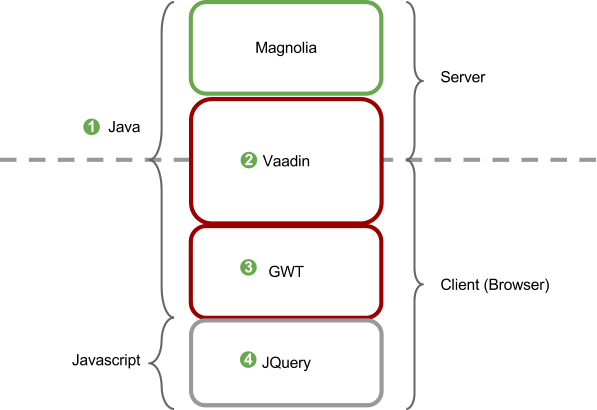
\includegraphics[width=\textwidth]{magnolia_stack.png}
	\caption{Magnolia CMS 5.0 technology stack}
	\label{fig:technology_stack}
\end{figure}

\section{A CMS vs an Application Framework}
First of all we should clarify the difference between a CMS and an application
framework. Most CMS's are built on top of an assumption about how the content
should be managed. Where as application frameworks make no assumptions about
that or even about what the content is. The power of an application framework is
in the set of basic capabilities it provides that allow to structure and manage
the data in any possible way. Magnolia 5.0 architecture proposal fits the
combination of two realms very well: while Magnolia core API's concentrate on
providing the best tools for website editors \cite{ux_andreas} let the
administration part of the CMS be built with an application framework that will
provide convenient ways to extend the system for developers. Such an approach
has a variety of benefits over the frameworks built in-house. First of all, this
would allow for adopting the best practices of application architecture design
by simply delegating the tasks to the application framework. The maintenance of
the system would be eased as well. The last but not the least benefit is the
smoother and easier adoption by Magnolia CMS community.

\section{Vaadin}
The Vaadin application framework is used for building the Magnolia 5.0
AdminCentral.
 
The core piece of the Vaadin Framework is the Java library designed to make
creation and maintenance of high quality web-based user interfaces easy. The key
idea in the server-driven programming model of Vaadin is that it lets you forget
the web and program user interfaces much like one would program any Java desktop
application with conventional toolkits such as AWT, Swing, or SWT \cite{BoV}.

As it is shown on the Figure \ref{fig:vaadin_arch} - the main part of Vaadin is
the server-side framework that runs within a Java application server on top of
the Java Servlet technology. A Vaadin application is stored in a servlet session
which typically handles the communication with various backend systems. An
Application also declares the user interfaces on the server side which are then
translated for different web browsers and rendered in the form of a JavaScript
program. The rendering and cross-compilation process of translating Java to
JavaScript is handled by GWT (a framework that we will discuss later on in this
chapter).

Being written completely in the Java language without and requiring no
additional configuration Vaadin integrates effortlessly with almost any other
Java technology. For example the dependency injection frameworks 
Spring and Google Guice. It also deploys deploys on almost any application server (e.g. JBoss,
GlassFish, Tomcat, Jetty etc). This means that Vaadin could easily be used with
Magnolia core API's out of the box.

Let us briefly study the architecture of the Vaadin framework.
\begin{figure}[H]
\begin{center}
  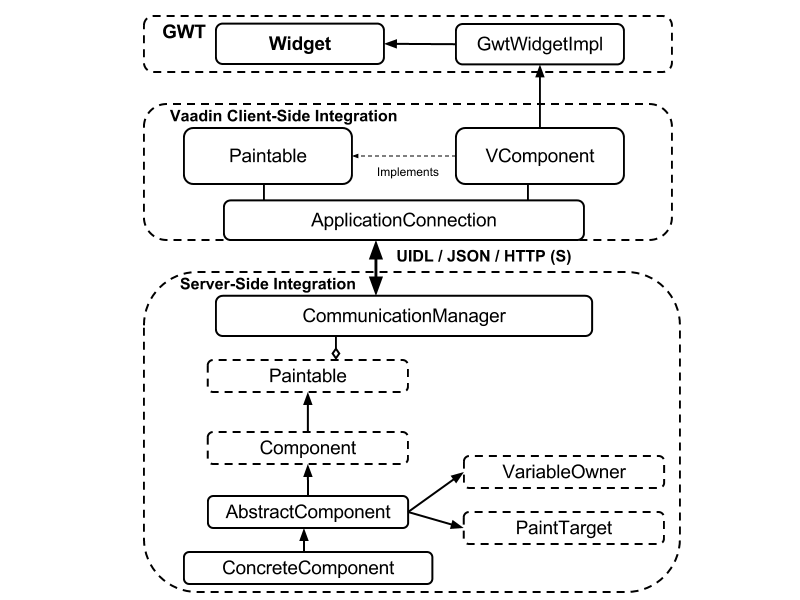
\includegraphics[width=\textwidth]{vaadin_architecture.png}
  \caption[labelInTOC]{Vaadin framework Architecture}
  \label{fig:vaadin_arch}
\end{center}
\end{figure}
 
\subsection{Servlet Level} 
An application that uses Vaadin runs as a servlet in a
Java web server, serving HTTP requests. The terminal adapter receives client
requests through the web server's Java Servlet API, and inteprets them to user
events for a particular session. Sessions are tracked using cookies. Events are
associated with UI components and delivered to the application, which handles
them with listeners. If the application logic makes changes to the server-side
UI components, the terminal adapter renders them in the web browser by
generating a response. The client-side engine running in the browser receives
the responses and uses them to make any necessary changes to the page in the
browser.

\subsection{Application level}.
The top level of a user application consists of an
application class that inherits \texttt{com.vaadin.Application}. It creates the
UI components (see below) it needs, receives events regarding them, and makes
necessary changes to the components.
For detailed information about inheriting the \texttt{Application} see \cite{BoV}.

\subsection{User Interface Components}
The user interface consists out of UI
components that are created and laid out by the application.
Each server-side component has a client-side counterpart, with which the user
interacts. The server-side components can serialize themselves over the client
connection using a terminal adapter. The client-side components, in turn, can
serialize user interaction back to the application, which is received in the
server-side components as events. The components relay these events to the
application logic. Most components are bound to a data source (see below). For a
complete description about the UI component architecture see \cite{BoV}.

\subsection{Client-Side Engine} The client-side Engine of Vaadin manages the
rendering in the web browser by using the Google Web Toolkit (GWT). It
communicates user interaction and UI changes to the server-side terminal adapter
by using the User Interface Definition Language (UIDL), a JavaScript Object
Notation (JSON) based language. The communications are made using asynchronous
HTTP or HTTPS requests.
\cite{BoV}.

\subsection{Terminal Adapter} Client-server communication in the Vaadin framework
is encapsulated into the so called Terminal Adapter concept. It is a mechanism
that typically manages the payload transfers between component client and server
counterparts while hiding the actual transport technology. Typically (in Vaadin
6) the underlying pipeline is the AJAX technology - the client side widgets fire
the events which are then transformed into variable changes by the
\texttt{com.vaadin.terminal.gwt.client.ApplicationConnection} class and sent to
server side where they are handled by the
\texttt{com.vaadin.terminal.gwt.server.CommunicationManager}. The
\texttt{CommunicationManager} class dispatches the changes to the corresponding
components which process them producing the response (the UIDL payload). As a
result the communication happens automatically and typically developers do not
have to take care about it unless they are building an extension for the Vaadin
framework.

\subsection{UIDL} The Terminal Adapter renders the user interface and its updates
to the Web page by means of the User Interface Definition Language (UIDL). The
UIDL communications are conducted over JavaScript Object Notation (JSON), which
is a lightweight data interchange format that is especially efficient for
interfacing with JavaScript-based AJAX code in the browser. \cite{BoV}.

\subsection{Events} User interaction with UI components creates events. The
lifecycle of an event typically starts with processing on the client side with
JavaScript. Then the event is passed all the way through the HTTP server,
terminal adapter, and finally - to the application instance and its user
component layers. \cite{BoV}.

\subsection{Themes} The user interface is a separator between presentation and
logic. While the UI logic is handled as Java code, the presentation is defined
in themes as Cascade Style Sheets (CSS). Vaadin provides a set of default
themes.
User themes can, in addition to style sheets, include HTML templates that define
custom layouts and other resources, such as images \cite{BoV}.
 

\subsection{Data Model} In addition to the user interface model, Vaadin provides
a data model for streamlining the data presented in UI components. By using the
data model, the user interface components can update the application data
directly, without the need for any control code. All the UI components use this
data model internally, but they can be bound to a separate data source as well.
For example, you can bind a table component to an SQL 
query response \cite{BoV}.In the case of the Magnolia CMS we will examine the
development of the \texttt{Container} implementation that binds to the Java Content
Repository.


\section{GWT}
Google Web Toolkit (GWT) is a development toolkit for building and optimizing
complex browser-based applications \cite{GWT}.
GWT is an open source framework developed by the Google corporation. The main
goal of the toolkit is to provide developers with an ability to write their
client side programs in Java without browser plugins or additional software.

\subsection{Compiler} 
The core of the Google Web Toolkit is a Java-to-JavaScript cross-compiler that
translates the Java program into highly optimized JavaScript code. The process
of cross-compilation involves the consequent building of Abstract Syntax Trees
(AST) that proceduraly formalizes Java code, optimizes it, translates to
JavaScript and then optimizes it again.
A possible drawback for the compiler is the time it requires to translate the
code. For a big projects this can take up to several minutes (even on powerful
machines with multi-core CPU's).

\subsection{Deferred Binding} 
Deferred binding is the crux of the GWT compiler. It is the process of
generating multiple chunks of JavaScript code each of which are later
served for different cases. The default case is the generation of different
versions of JS output (in order to overcome the browser dependent
peculiarities). It means that if some cases have to be handled differently e.g.
in FireFox and Internet Explorer, the developer does not have to use conditional
statements in his code but rather instruct the compiler on which logic to use
for each option. Such an approach reduces the amount of JavaScript code sent
over the network and improves code clarity and quality. Deferred Binding allows
for easier implementation of localization, resource handling and, what is very
important for Magnolia 5, automatic handling in cases of a visit from a mobile
devices\cite{def_bind}.

\subsection{JSNI}
Just like it is possible to inject C code into a Java program (Java Native
Interface or JNI) it is possible to inject the JavaScript code parts into the
GWT classes.

This approach brings many benefits for the GWT developers\cite{jsni}:
\begin{itemize} 
	\item Implement a Java method directly in JavaScript.
	\item Call from JavaScript code into Java code and vice-versa.
	\item Wrap type-safe Java method signatures around existing JavaScript.
	\item Throw exceptions across Java/JavaScript boundaries.
	\item Read and write Java fields from JavaScript.
	\item Use a development mode to debug both Java source (with a Java debugger) and JavaScript (with a script debugger).
\end{itemize}
In fact most of the low level GWT functionality is written with JSNI. It is
worth mentioning that irrational usage of JSNI can spawn a variety of issue like
more complicated portability across browsers, higher potential for memory leaks
than native GWT code and optimization issues \cite{jsni}. Nevertheless Magnolia
5.0 embraces it for integration of JavaScript libraries and API's and
development of widgets that would require more fine grained event handling.
[TODO - ADD CODE SNIPPETS AND EXPLANATION OF TYPE-MAPPING]

\subsection{Widgets and Events} 
The building block of GWT applications is the Widget
(\texttt{com.google.gwt.user.client.ui.Widget}).
Widget is typically a wrapper around a set of Document Object Model (DOM)
elements with business logic methods and event handlers. GWT is shipped with a
powerful event system which is based on the EventBus pattern. It allows for
building both user-defined events as well as the wrappers for the native DOM
events. GWT's event system carefully handles the cases with potential of memory
leaks \cite{gwt_memory_leaks} which are the source of various complex issue of
the programs written in plain Javascript. All this features are perfectly useful
for building readable and loosely coupled UI interfaces on the client side.

\section{JQuery}
JQuery is a popular JavaScript library which is so popular that it is probably
the first thing the name of the language is associated with. JQuery simplifies
HTML document traversing, event handling, animating, AJAX interactions and many
other areas of web development \cite{jquery}. 

JQuery is a base framework for a wide range of web project's front-end (e.g.
Wikipedia \cite{jquery}). However, in the case of Magnolia 5.0 project the
leading role in client-side development is devoted to GWT. Unfortunatelly, GWT
does not provide the solution for all the problems, a front-end developer might face.
One of such issues is a support for CSS3 transitions \cite{ccs3_transitions}.
Transitions API is not yet finally standardized and not fully cross-platform
which makes it hard to support with GWT. JQuery provides several convenient
approaches for adopting CSS3 transitions in the project. Due to \emph{JSNI}
mechanism it is possible to integrate JQuery with GWT and fulfill the gaps in
functionality of the latter. 
 
\section{Why Vaadin?}
\paragraph {Server Side Execution}
While execution of the UI events on the server side is quite controversial it
has several crucial benefits for a CMS development as CMS itself is mostly a
server side technology \cite{why_vaadin_philipp}.

\begin{itemize}
  \item Reflection can be used. While GWT code can't use reflection server side
  code can. This is for instance very helpful when 
  XML defined Magnolia entities are transformed into Java objects.

  \item Security is endorsed in many ways. Access Control Lists (ACL) can be
  easily used where ever needed. Additionally, having all the logic on the
  server side makes it next to impossible to break into the code and violate
  restrictions on the client side.

  \item Less web services. The UI is built on the server, but rendered on the
  client. So there is no need to define additional services for receiving dialog
  and tree descriptors. It is only required to expose the content related to the
  stateless Representation State Transfer (REST) services.

  \item Less GWT compilation is needed. Unless another module is added with its
  own client side implementation, the compilation should be done only once as to
  preserve development fluency. Agility is also increased by out-of-the-box
  support for any other JVM languages like Scala or Groovy. The latter of which
  is highly adopted in Magnolia.

  \item Testing concerns. Having all the logic on the server makes it easy to
  set up unit testing. Not only testing of for purely server side concepts like
  services, data storage connections and data processing, but also for testing
  of UI classes (to some certain extent). This is very important because, for
  instance, event handling in a complex application might become quite a fragile
  and sensitive task.
   
  \item Magnolia API. The Magnolia API can be fully exploited and no Data
  Transfer Objects (DTO) are required due to the fact that the UI logic is
  integrated with Magnolia API on the server side.

  \item Collaboration. The Magnolia and Vaadin communities and the backing
  companies are looking forward to support this collaboration and to help each
  other to make this successful.
  
\end{itemize}

\section{Possible Challenges}
The biggest cause of issues for the aforedescribed technology stack is the
performance. Being a server-side centristic application Magnolia 5 has to have
an architecture that finds a balance between a good and feature rich UI and
stable and scalable responsiveness. This could be described as several
requirements for the system:

\begin{itemize}
  \item Efficient data management. A proper integration of the JCR API and the
  Vaadin Data API is required. Due to memory consumption restrictions it is
  crucial that the smallest achievable amount of actual data is stored in memory
  at the same time. On the other hand, some caching or paging is needed in order
  to have most of the actual data accessible.
  
  \item [TODO: rephrase] Despite the fact that Vaadin has a big UI component
  bundle shipped with it - many of them have some sort of overhead:
  either rather complex DOM structure that is optimized for the versatility not
  crucial for considered project or too eager client-sever communication. This
  makes a demand for a row of additional components to be developed for Magnolia
  5.0 project.

  \item Transitions. Transitions between views is one of the key points of an
  interface optimized for good user experience. Smooth and logical transitions
  make the process of navigation more understandable and enjoyable. However,
  Vaadin does not support the transitions between the views out of the box.
  However, the existing solutions are server-side handled and they create an
  unnecessary communication spike on the back-end.
  
  \item Mobile support. Vaadin framework has an extension called the TouchKit
  which supposedly provides the functionality for mobile web applications.
  However, it was mainly created to support development of native-looking web
  applications and does not provide a framework with the capabilities for
  handling gestures and touch events. Thus, it is required to either build a new
  or integrate the existing solution to overcome this issue.
\end{itemize} 

\pagebreak

\chapter{Magnolia 5.0 AdminCentral Module Architecture}
\label{architecture}

The biggest part of the Magnolia 5.0 project is the design and development of
the AdminCentral module - a replacement for the former \emph{AdminInterface}
module. Improved user interface is one of the major targets for AdminCentral
module.

However, the role of AdminCentral is supposed to go far beyond the UI
shell. It is the point of intersection between most of the other modules, a
framework that allows to create complex abstractions on top of their
functionality and provide an easy way to set up communication between them.
In order to fulfill the aforementioned design requirements for extensibility and
mobile platforms support - it was decided to emulate the environment of an
operating system for CMS administration. The resemblence is of course supposed
to be metaphorical, design-wise. The main idea is to have an environment with a
chrome and applications that run inside of it. Such a pattern allows for
creating the additional functionality by merely developing another application.
In order to maintain the common look and feel for all types of platforms the
mobile-like way of UI arrangement was chosen: Single Document Interface (SDI)
with a dashboard and the applications that consume the whole viewport one at a
time.

the AdminCentral is to provide a framework for the applications: both
initial and additional apps must be equally easy to develop, the amount of the
boilerpalte code has to be minimal and the least amount of programming skills
should be required.

The role of \emph{Vaadin} framework in the \emph{AdminCentral} is to make it
possible to achive the compromise between the rich UI and the development
clearness and simplicity.
With Vaadin it is possible to design the entire application development system
completely on the server-side: the user interface can be generated directly form
the configuration templates kept in the storage (JCR) and the powerful
client-server communication mechanism can be used for emulating the navigation
 (based on the browser-fragments).
\section{Architecture Overview}

\begin{figure}[H] \centering 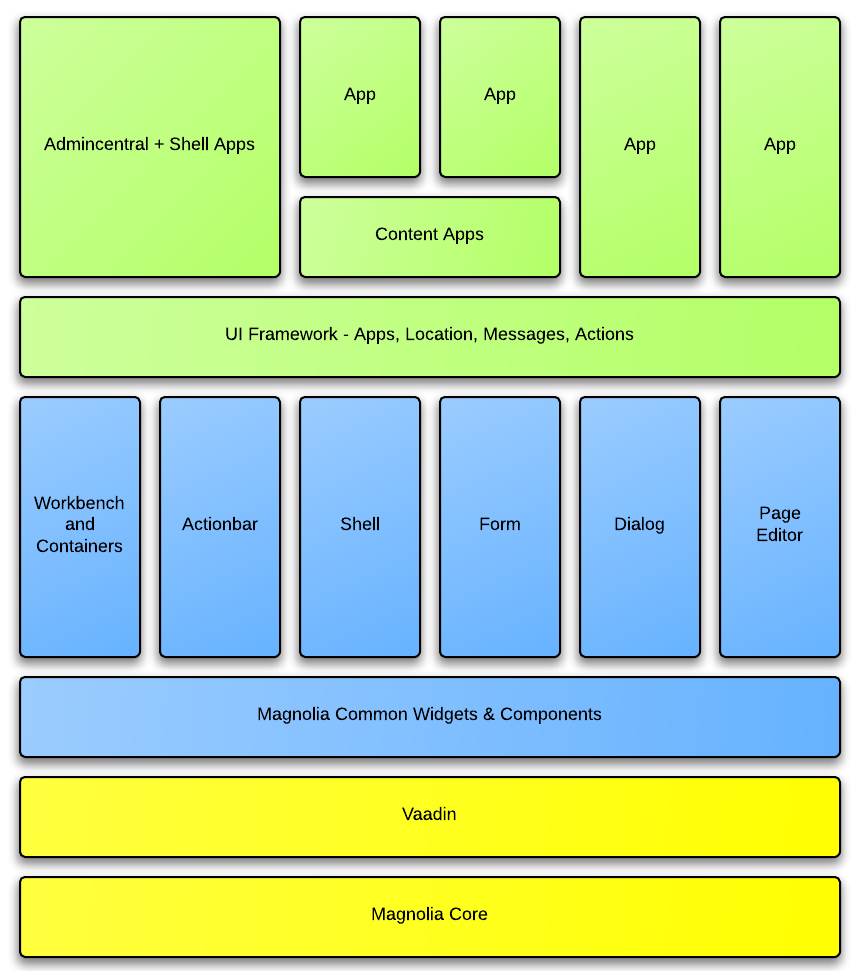
\includegraphics[width=\textwidth]{architecture_layers.png}
	\caption{High-level architecture overview}
	\label{fig:architecture_overview}
\end{figure}

Firgure ~\ref{fig:architecture_overview} displays the structure of the project
architecture. The main goal of a such architecture design is to provide a set of loosely
coupled components and interfaces. The block structure means that every block is
a separate Magnolia CMS module which encapsulates a logical part of the system.
The firgure ~\ref{fig:architecture_overview} also describes the dependency
hierarchy of the project: the parts of the system can only depend on the blocks
that belong to the layer that resides below in the diagram. This means that most
low-level tiers of the architecture are core Magnolia API and plain Vaadin
components and interfaces, whereas the top-level parts are apps - parts of the
system actually visible to an end-user. Apps can re-use any API and frameworks
present in the system. Let us briefly discuss the features of all the layes of
the architecture.

\subsection{Magnolia Core API and Vaadin} 
  The main two frameworks used in the system
  provide a low-level foundation of Magnolia AdminCentral module. Magnolia Core
  API enables interfaces and utilities for accessing JCR, dependency injection
  functionality, tools for localization etc. Vaadin serves as a platform for the
  Magnolia AdminCentral web-application and abstract building blocks
  (Components) for moe specific parts of teh system.
\subsection{Magnolia Common Widgets and Components} 
  This layer of the system aggregates the essential re-usable components built on top of the core
  frameworks. Such components include, for instance, the page editor - the
  What-You-See-Is-What-You-Get (WYSIWYG) utility for modifying the website
  pages. Common Components layer also includes the data management structures
  such as JCRContainer.
\subsection{UIFramework} 
  UIFramework layer provides the foundation for the apps,
  such as base classes and interfaces, action-execution mechanisms and message
  exchange infrastructure. UIFramework also contains the fundamental
  communication framework for the entire AdminCentral web application, which is
  called Location Framework.
\subsection{AdminCentral and apps}
  Finally, the top-most architecture layer is reserved for apps and AdminCentral
  web application. An app represents a logically and functionally consistent
  unit that allows for conducting certain operations on the contnet and/or the
  essentail workflow utilities.

In the current chapter we will mostly discuss the concept of the UIFramework in
detail. The importance of UIFramewor cannot be overestimated because it is a connection
point between the core API's and comonents and the apps. We will pay additional
attention to the app-framework as well. The following chapter
(\ref{implementation}) will highlight the implementation details of the most
crucial components from the common widgets layer.

\section{Technology Stack Roles Distribution} 
Before starting to explore the parts of Manolia 5.0 architecture in details and
analyzing how they solve the problems stated in \ref{thesis_problems} it is
important to clarify the communication relationships between the frameworks used
in the project. We also need to define which framework acts on the server-side
and which - on the client-side. Let us consider the high-level outline of
project's structure displayed on the figure \ref{fig:architecture}:

\begin{figure}[H] \centering 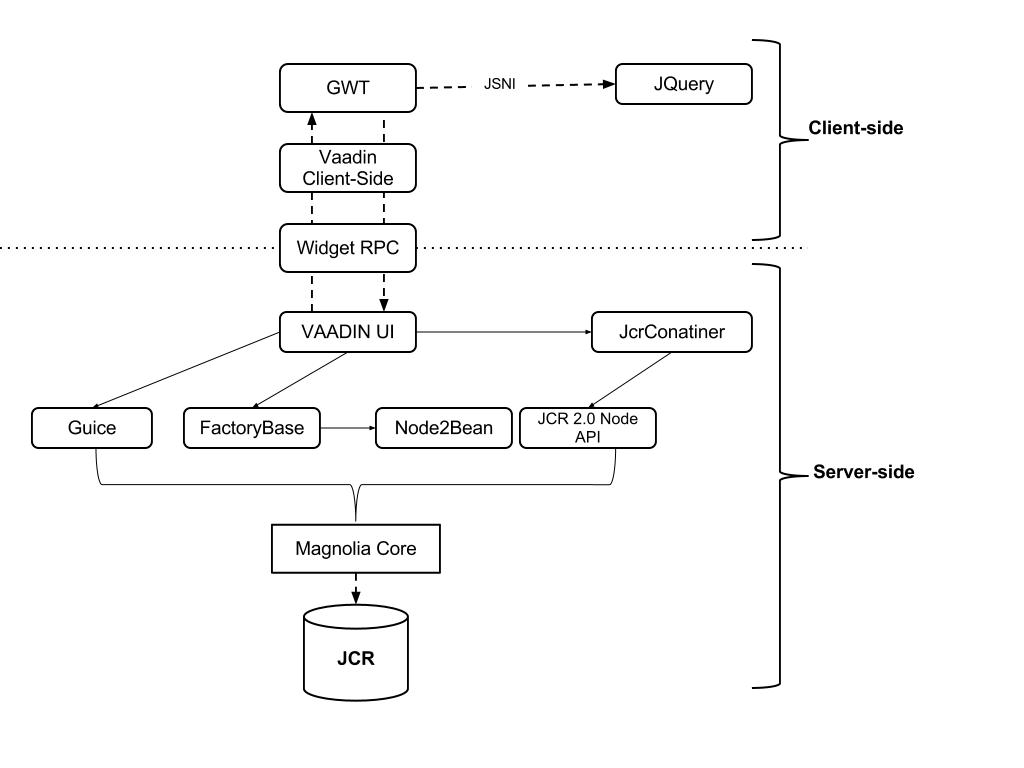
\includegraphics[width=\textwidth]{architecture.jpg}
	\caption{Magnolia CMS 5.0 Architecture}
	\label{fig:architecture}
\end{figure}

\paragraph{JCR} repository is at the lowest level of the hierarchy and stores
not only the content and templates but also all the configuration for the
system:
\begin{itemize}
  \item The structure of the user interface building blocks.
  \item Registries of the functionality units used within the system and the way
  they are accessible for the user.
  \item Binding between the action definitions that can be performed on the
  nodes and their implementation.
\end{itemize}

\paragraph{Magnolia Core} API's provide the low-level communication mechanism of
interaction with JCR and implementation for the various patterns that can be
re-used in the project. The most important parts of it include for instance the
API for querying the JCR and Node2Bean that allows for projecting the nodes to
Java Beans transparently to the developer. Another crucial framework provided by
the Magnolia Core is the Dependency Injection (DI) functionality based on Google Guice
\cite{google_guice}. The main strength of this framework is that allows to
define the mapping between the interface and the implementation of the
components right in a module descriptor - all the other configuration is done
internally and the developer does not have to take care of it, it is usually even
not necessary to know what DI mechanism actually provides the fucntionality.

\paragraph{Vaadin} layer is based on top of JCR and Magnolia Core API's. It
plays a role of the foundation for the AdminCentral web application. Vaadin
generates all the components and views of the system based on the information
provided by the configuraion. The datasources for the components are normally
provided in a form of the \texttt{JcrContainer} which is an implementation of
the Vaadin's \texttt{Conatiner} interface based on top of the JCR Node API.
Vaadin resides in the top level of the server-side architecture. 

\paragraph{Vaadin} interacts with the client-side by means of its core
communication mechanism (UIDL, see \ref{chapter_tech_stack}) and by means of an
additional API provided by the WidgetRPC add-on. The latter is used in order to
improve the clearness and simplicity of communication. UIDL
communication allows for passing the numerous variables between the client and
the server, resulting in rather complex code structures that analyse the
incoming changes.

Contrary to the plain UIDL, WidgetRPC allows for building the communication
interfaces and mutually call the methods between the component's counterpart,
making the conversation between them more fine-grained and roust.

Vaadin client-side part is responsible for handling both ways if the
communication and also controls the resuting UI presentation.

\paragraph{Finally, GWT} is responsible to produce the views on top the commands
and instructions that are coming through the Vaadin's client-side engine.
Whereas the simpliest vaadin applicaton does not require the programmer to engage
GWT into the development (core Vaadin's widgetset could be enough) Magnolia 5.0
project requires a variety of the custom components to be built so that the
resulting interface gets all the necessary components without significant
overhead caused by adopting the ones from the core. In order to increase the
performance and to provide some complex UI effects the JQuery library was
incorporated into the project's client-side ramework. The access to JQuery can
be done directly from GWT.

\section{Location Framework}
We will start a detailed discussion about the UIFramework with an in-depth look
into the structure of the AdminCentral web application and its backbone - the
\emph{Location Framework}.

As it was discussed in the beginning of the chapter AdminCentral web application
is based on Vaadin framework. According to chapter \ref{chapter_tech_stack}
Vaadin applications work on top of Java Servlet API and any logic that is
executed within application is triggered by user input within the web browser.
An application is responsible for loading, displaying and closing the proper
views on a screen in response on the various events. Typically Vaadin
application would create, attach or detach components, set up the references
between them and update the states of components.

We have stated in chapter \ref{thesis_problems} that one of the most crucial
goals of the project is to provide an extensible and highly-customizable user
interface allowing for adding and removing the functional components on demand.
This requirement implies that AdminCentral web application must obtain an
abstact framework for the state management. An obvious solution would be to
provide mappings between possible URL's and the views. Such mappings should be
easilly customizable and the views should be possible to be pre-created as well
as generated on the fly (e.g. - based on the parameters of the query). All these
statements bring us to the navigation management framework called \emph{Location
Framework}.

Navigation handling is one of the most common problems that Rich Internet
Applications (RIA) developers face. For instance - dealing with poor support of
the browsers' history. The source of the problem is the fact that the frameworks
like GWT usually provide capabilities for building the single-paged applications
with an only one highly dynamic page that generates HTML-views according to
UI-logic. In such situations teh browser is not responsible for tracking the
navigation. For instance if a user presses the "back" button he will most likely
navigate away from the application, which is usually not the desired behavior.
However, this problem is possible to handle by means of a framework. GWT, for
instance, provides the API for the interaction with a web-browser history based
on fragments.
Fragment is a part of a URL after the hash sign (\#). Changing a URL-fragment
does not trigger a browser refresh, so a framework can provide the track of an
application internal navigation history by manually pushing the items into
browser history \cite{gwt_historian}.  Let us consider an example:
\url{http://www.example.com/example_app#view1}

In this example everything before the hash sign \texttt{(\#)} is the example-app
URL and the \texttt{view1} is the identifier of some application UI state. If a
user navigates to this URL in a browser GWT will fire an internal event and the
application client-side logic will determine which user interface parts to
display.

However, URL fragment is just a tool that could be used for navigation.The main
problem is how to effectively map the multiple views that a complex Rich
Internet Application might provide to the corresponding URL fragments. It also
should be possible to serialize the state of the views in the fragment and many
others.
For native GWT applications the framework team has provided a rather flexible
and useful sub-framework called Activities and Places framework
\cite{activities_places}.

Activities and Places is a design pattern for structuring the navigation in a
user interface. The parts of an application are its activities and they can be
reached by activating their respective place. For web applications a place is
derived from the browser URL allowing a section of the application to be
bookmarked. As the user interacts with the application the browser URL changes
in response to place changes.

Activities and Places framework is widely used by the GWT community. However,
for a server-side oriented application like Magnolia 5.0 AdminCentral it would
be impossible to use it for navigation, as the client-side is rather thin. As a
consequence it was decided by the development team to port the framework to the
server-side and adopt it for Vaadin-based applications. The resulting concept is
called the Location framework. The name location was chosen to substitute the
term place because it reflects the web nature of the application better: the
current URL of a RIA or a site is obtained by calling \texttt{window.location}
in JavaScript.  Let us consider the Locations framework in details.

\subsection{Location}

\begin{figure}[H] \centering 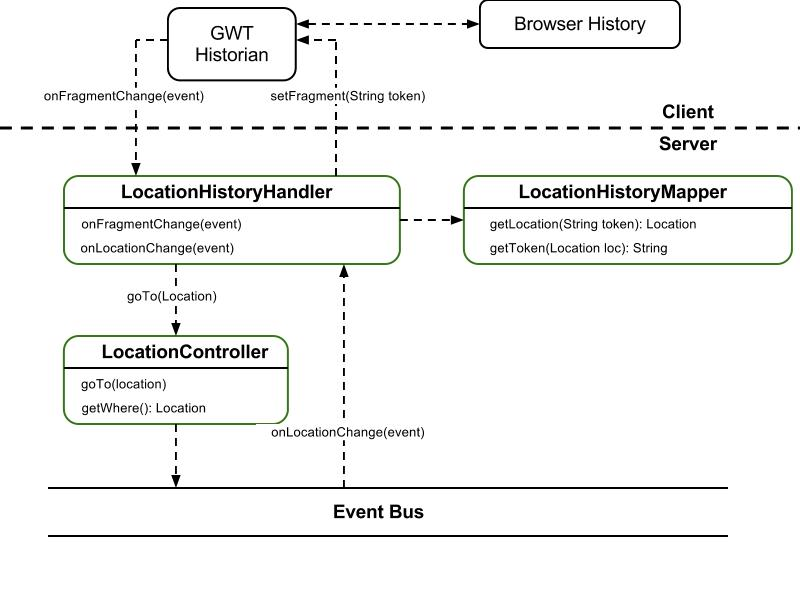
\includegraphics[width=\textwidth]{location_arch.jpg}
	\caption{Location framework pt.1}
	\label{fig:location_arch}
\end{figure}

\subsubsection{Location} 
Location is a data transfer interface between the server-side and
the browser history. It is capable of deserializing a fragment string into a 
Plain Old Java Object (POJO). That POJO in turn can serialize itself into a
valid URL fragment string.

\subsubsection{Event Bus}
 The backbone of the Location framework is the EventBus
(\emph{TODO Consider EventBus pattern appendix}). One global event bus acts as a communication
channel between other parts of the framework. For instance, it gets notified of
the fragment change from the client-side and triggers the user interface
change sequence. On the other hand, when a UI update is initiated on the
server-side due to some user input and an application navigates to a new
location, an event bus propagates the new location to all the interested
parties. The location is eventually transformed into the fragment and ends up on
the client-side in the browser history.

\subsubsection{Location Controller} \texttt{LocationController} is a singleton
(/*consider appendix*/) object that handles navigation between locations and keeps
current location. \texttt{LocationController} is tightly
connected with the event bus:
the latter accepts the listeners and transmits the events fired by the
controller. In order to perform navigation to a different location through the
\texttt{LocationController} one has to simply call the following:

\begin{lstlisting}
	locationContoller.goTo(location);
\end{lstlisting}

Such a call changes and controller's current location and causes it to emit a
LocationChangeEvent on the event bus. A good example of a
\texttt{LocationChangeEvent} handler would be some kind of a UI manager that
would find and/or construct the appropriate view depending on a location.

\subsubsection{LocationHistoryHandler and LocationHistoryMapper} 
Another entity that handles the \texttt{LocationChangeEvents} is
\texttt{LocationHistoryHandler}.
It is the connection point between the framework and the web browser. It is
capable of converting the location into a string (URL fragment) and vice-versa -
obtaining a location by a fragment. However, \texttt{LocationHistoryHandler}
does not accomplish these tasks on its own rather than that - delegating the
implementations of search and conversion to a \texttt{LocationHistoryMapper}.
\texttt{LocationHistoryMapper} as it is stated in its title maps the unique
history fragments to corresponding locations in a bi-directional way.


\subsection{Activities and ActivityManagers}
\begin{figure}[H] \centering 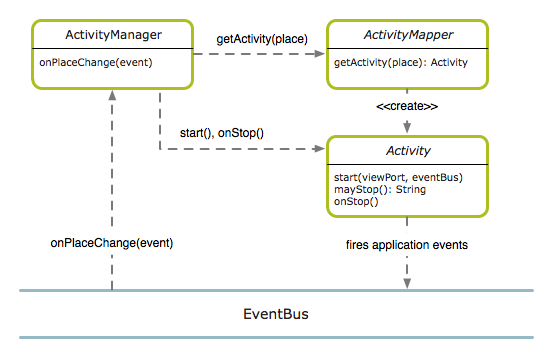
\includegraphics[width=\textwidth]{activities.png}
	\caption{Location framework pt.2}
	\label{fig:location_arch}
\end{figure}

\subsubsection{Activity}
\texttt{Activity} is the concept of the original framework from Google Web
Toolkit. Its main purpose is similar to the role of the Presenter in
Model-View-Presenter pattern which will be discussed later in the current
chapter (see \ref{MVP}). Provided with a state snapshot stored in a location and
a viewport for rendering an \texttt{Activity} is able to handle state,
initialize, update, load and unload the \texttt{View}\cite{activities_places}.
\texttt{Activity} is also able to notify the other objects (e.g. a different
\texttt{Activity}) about its internal events through the framework's
\texttt{EventBus}.
 
\subsubsection{ActivityManager and ActivityMapper}
\texttt{ActivityManager} and \texttt{ActivityMapper} classes purpose is to
resolve an
\texttt{Activity} that corresponds to an incoming \texttt{Location}.
\texttt{ActivityManager} subscribes to an \texttt{EventBus} and awaits for new
\texttt{Locations}.An \texttt{ActivityMapper} is used as a registry that mapps 
an \texttt{Activity} to a \texttt{Location}.

In Locations framework the role of the Activities is played by the
\emph{Apps} and the job of \texttt{ActivityManager}
and \texttt{ActivityMapper} is done by an \texttt{AppController} (see \ref{section_apps}).


 
\section{Model-View-Presenter}
\label{MVP}
As we have discussed before - \emph{Location Framework} provides an abstract and
convenient functionality to map the application logic to the changes triggered
by means of the URL fragments changes. We mentioned Model-View-Presenter (MVP)
pattern in that discussion as a connector between the URL fragment and the
actual \texttt{View}.

However, this is not the only use case of this pattern within the project: it
appears to be useful when separation between user interface and its presentation
logic is required. Let us explore the concept of the Model-View-Presenter
pattern and the ways of its adoption in Magnolia 5.0 application.

Model-View-Presenter (MVP) pattern is one of the cornerstone patterns of
Magnolia 5.0 user interface. A lot like the classic Model-View-Controller (MVC)
pattern MVP aims for the separation of user interface implementation from the
presentation logic.
\begin{figure}[H] \centering 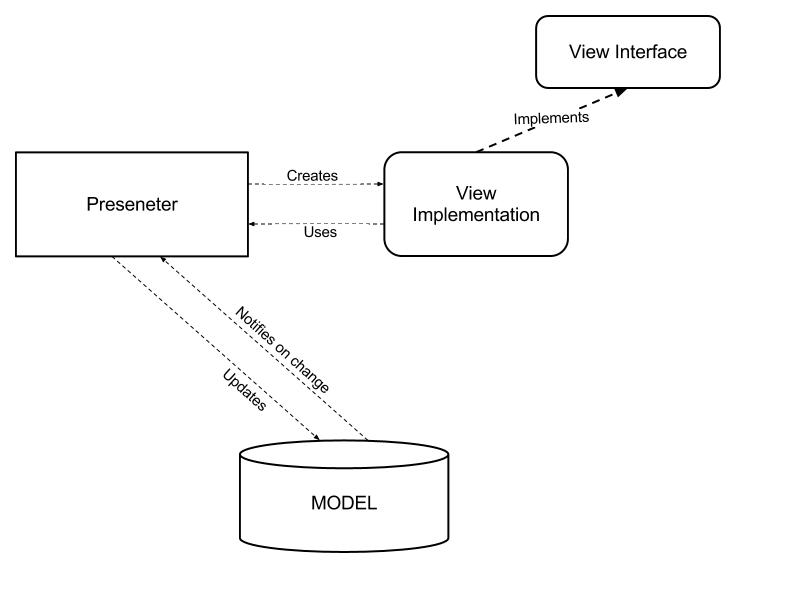
\includegraphics[width=\textwidth,
height=\textheight, keepaspectratio]{mvp.jpg}
	\caption{Model-View-Presenter}
	\label{fig:mvp}
\end{figure}
Advantages that Model-View-Presenter pattern offers are:
\begin{itemize}
  \item Clear design with completely separated handling of UI events form the actual handlers logic.
  \item Possibility to re-use interfaces of the views and presenters interfaces for different implementations.
  \item Separated test for the UI and for logic. 
\end{itemize}

\subsection{Presenter} Presenter exposes an interface that contains methods for all the actions that could be triggered in a view
like search, filtering, update etc. As an action is invoked by the view the presenter executes the necessary operation,
accessing model if needed. After that the presenter updates the view accordingly. Presenter is also responsible for
reaction on the changes of model not triggered by the current view.

\subsection{View} The view is logically clear composition of a set of user interface components that displays and/or gathers data
from the user. The view interface exposes all the methods that a presenter might need to assemble and steer it (e.g.
access to the parts of the view, getters/setters for some fields etc.). Ideally the view is not supposed to be bound to
any UI technology completely concealing its implementation from the presenter, so the presenter tells the view what to
do, whereas it is up to the view to decide how to do it. In case of Magnolia 5.0, however, we will break this rule and
for almost all the cases oblige the view to expose itself as a Vaadin component (because Vaadin is the only UI
technology used on the server-side).

\subsection{Model} Model is a data source used by a presenter. In Magnolia
CMS model is obviously a JCR repository. However, direct
access to JCR would be quite cumbersome and inefficient, so the actual communication with presenters in Magnolia 5.0
happens through the Vaadin data binding layer - a special JCR container, which will be discussed in the following chapter.

As it was already mentioned, MVP resembles Model-View-Controller pattern. However, in classic MVC the controller has to 
listen to both the View and the Model. This means, for instance, that the button click and text change handlers are registered
there. In MVP, on the other hand, the presenter only implmenets a set of certain functions that are invoked by the view.
Thus, MVP provides better decoupling between the view and the presentation. 

Besides already mentioned specialties of MVP use in Magnolia 5.0 (like a constraint to Vaadin) it is worth mentioning
that the main responsibilities are distributed differently than usual. Normally it is the job of the view to initialize
the presenter whereas in Magnolia 5.0 it is vice versa and the presenter creates the view. This difference is caused by
how the user interface is persisted in the back-end: JCR configuration repository contains only the information how to
build the UI which is a description of the presenter. Later when the user navigates to some specific view a pre-created
presenter instantiates the actual UI component.
\section{Configuration in Magnolia CMS}
By means of the \emph{Location Framework} and \emph{MVP} pattern which were
described before we have defined a foundation for an abstract loosely coupled
system which is capable loading, rendering and disposing some components.
Adding a new functionality in such a system would only require to
implement its logic and to add the proper mapping, so the system would load the
component on demand. However, the end developer should not be required to change
the source files or mapping configuration manually. Instead there should be an
interface by means of which the developer would interact with the system and
alter its state. In the current section we will analyze the approach of a
high-level definition mechanism used in Magnolia 5.0.

Configuration mechanism is an essential feature of many software products. It
enhances the flexibility and extensibility in the sense that the person without
deep knowledge of the system internals can alter its behavior, re-arrange and
customize its parts. 

Magnolia CMS is also configurable by means of XML. Each module has an XML
descriptor containing all the properties needed for its description. An example
of a configurable component could be a registry of the forms with fields which
would be represented with a set of XML nodes with properties and sub-nodes for
fields types, captions, default values, validators etc. 

Most of Magnolia CMS configuration files are kept within \emph{config}
workspace. Displaying this workspace in a form of editable tree would allow the
user to modify the components visually in real time as long as the system
instantly reacts on those changes.
There are several techniques in Magnolia CMS that are used for applying the
configuration. The main two concepts are \emph{observation} and \emph{Node2Bean}.

\paragraph{Observation} is a feature of JCR that allows for subscribing to the
changes in a workspace. Observing applications can monitor and react on those
changes whenever the persistent operation is made in JCR. This feature has found
various ways of applications in Magnolia CMS. For instance, one of the most
important ways is the foundation for the factory-based [TODO: consider factory
appendix] structures: some sort of bindings are stored in a workspace in a form
of the registry which is later used in the factory to produce the actual objects.

\paragraph{Node2Bean} is used to convert the JCR nodes into the Java objects. 

By means of Java Reflection (introspection mechanism) Node2Bean binds the the
fields of a Java Bean to the corresponding configuration properties (if such are
available) through the bean's "setter" and "adder" methods. Node2Bean can
support all possible data types:
\begin{itemize}
  \item Simple data types like \texttt{String, int, long, float, double, boolean}.
  \item Collections with String values or other data types by specifying a class property.
  \item Maps with keys and values as Strings or other data types by specifying a class property.
  \item Complex classes can be mapped with Node2Bean by means of the sub-nodes
  which follow the same rules and restrictions.
\end{itemize}

Let us consider an example of using Node2Bean:

\begin{figure}[H]
	\centering
	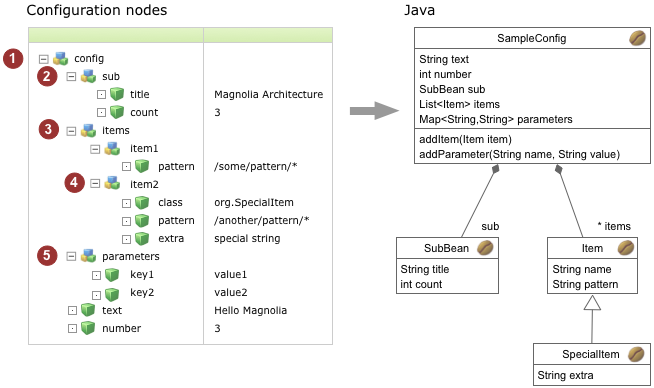
\includegraphics[width=\textwidth]{node_to_bean.png}
	\caption{Node2Bean mapping example}
	\label{fig:node2bean}
\end{figure}

Numbered items:

\begin{itemize}
  \item config: Entry point of the transformation. In the module descriptor
  \texttt{SampleConfig} class is used. Set text and number properties.
  \item sub: Sub bean. The class is determined using reflection if it is not
  explicitly defined.
  \item items: Collection. The corresponding add method is used to determine the
  class and populate the collection if existing.
  \item item2: Special item with its own class and additional properties.
  \item parameters: Collection of key-value pairs.
\end{itemize}

\section{It Is All About Apps}
\label{section_apps}
Magnolia 5.0 introduces applications of simply \emph{apps} to content
management. An \emph{app} stands for the configurable, pluggable unit which
encapsulates some certain functionality that typically operates over the data
stored in the JCR repository.
Magnolia 5.0 comes with a special framework for app management. This framework
is integrated with Magnolia CMS configuration mechanism which provides the
data required to start an app and Location Framework which triggers various
events causing app load, unload and navigation. 
There are two types of apps in Magnolia 5.0 - besides of apps of a regular type
(e.g for page editing or workspace browsing) there are special administrative so
called \emph{shell-apps}.

\subsection{Apps} An app is \emph{a tool with a very narrowly focused interface
enabling CMS users to work on one set of closely related tasks or one specific
set of data. An app does not necessarily work on a single, physical data set
(e.g. the pages of a site), but may cover multiple physical data sets required
to solve the task it covers.} \cite{maui_apps}. It is worth mentioning that in
case of Magnolia 5.0 app is not an application per se but rather a concept of a
user interface metaphor.

\subsection{App Framework}
The \emph{App Framework} is a name for Magnolia 5 functionality that manages
apps. This involves interaction with Magnolia CMS configuration mechanism:
handling the app registry and reacting on changes in app configuration.
It also controls an app life-cycle events such as starting, displaying, and
stopping an app \cite{wiki_app_framework}. Finally, the App Framework keeps the contexts of loaded apps,
maintaining their state and order.

\subsubsection{App Configuration}
The primary configuation of the apps is done by means of the
\texttt{AppDescriptor} class. \texttt{AppDescriptor} is a simple Plain Old Java
Object (POJO) that holds the meta information like the app name, label and its
icon. A descriptor also carries the name of a class that actually implements the
app and a list of \emph{sub-app} descriptors. A \emph{sub-app} is an entity that
implements the part of an app functionality. The \texttt{SubAppDescriptor} class
resembles an analogous for the app except for the fact the sub-app is a terminal
structure, so it has no child descriptors. 

In order to provide a higher level configuration mechanism for apps it is
possible to describe App descriptors in JCR inside the \emph{config} workspace.
As the Magnolia CMS web application starts up the descriptors are mapped to Java
classes by means of the Node2Bean mechanism:

\begin{figure}[H] \centering 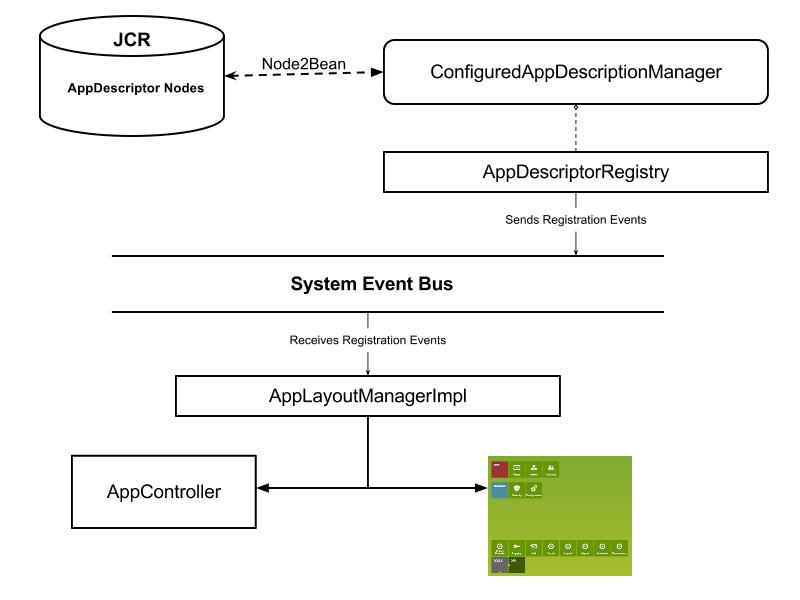
\includegraphics[width=\textwidth]{app_configuration.jpg}
	\caption{Registration of Apps.}
	\label{fig:app_registry}
\end{figure}

An instance of the \texttt{ConfiguredAppDescriptorManager} obsreves the changes 
in \emph{config} workspace and translates the JCR nodes that stand for the app descriptors to 
the objects of type \texttt{AppDescriptor}.

The scanned descriptors are then placed into the \texttt{AppDescriptorRegistry}
which fires the corresponding events for registration, deregistration or update.
The main receiver of such kind of events is an implementor of the so called
\texttt{AppLayoutManager} class. The purpose of this class is to maintain the
order of registered apps and to display them properly in the user interface (in
\emph{AppLauncher} shell-app) and to make them available to the navigation
system (the app controllers).

\begin{figure}[H] \centering 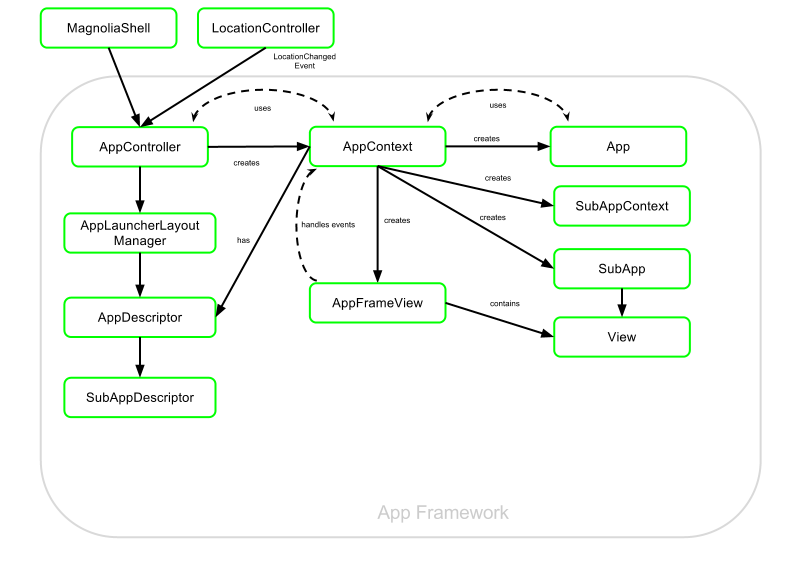
\includegraphics[width=\textwidth]{app_controller.png}
	\caption{App Context Management}
	\label{fig:app_context}
\end{figure}

\subsubsection{App Controllers and App Context.} The cornerstones of the \emph{App Framework} are the two
controller objects: \texttt{AppController} and \texttt{ShellAppController}.
These two objects play a similar role as \texttt{ActivityManager} in the original 
Places framework of GWT and apps are the analogues of \texttt{Activity}.
Controllers are subscribed to \texttt{LocationChangeEvent}'s. Based on the
incoming \texttt{Location}s either of two controllers retreives an app context.
\texttt{AppContext} is the class that holds the state of an app that is up and
running.

\begin{lstlisting}
public interface AppContext 
{
    void openSubApp(Location location);
    void start(Location location);
    void stop();
    void onLocationUpdate(Location newLocation);
    
    AppDescriptor getAppDescriptor();
    App getApp();
    
    View getView();
    String getName();    
    String mayStop();
}
\end{lstlisting}

As it is visible from the aforementioned fragment of an interface -
\texttt{AppContext} is able to react on \texttt{Location} changes. The
implementor of an interfaces typicaly conducts it by starting the app or one of
its sub-apps. An \texttt{AppContext} allocates the view component that would
host a new app (typically it is a tab-sheet component). It is also responsible
for providing all the neccessary paramteres to a newly created app or sub-app,
like dependency injector, reference to the context itself (so that the app could
indirectly communicate to the \emph{App Framework}) and location.

As the \texttt{start(\ldots)} method is called an \texttt{AppContext}
instantiates the sub-class of the \texttt{App} interface declared in the app
descriptor.

The \texttt{App} sub-class is basically a \emph{presenter} for a concrete app
implementation. We will cover the examples of app development in the
implementation chapter.

\subsection{Shell Apps.} There are three and only three shell apps that are
responsible for administration functions of the system. Those are called
\emph{AppLauncher}, \emph{Pulse} and \emph{Favorites}. \emph{AppLauncher} is a
dashboard with app icons allowing for starting apps and navigating between them.
\emph{Pulse} is an area that contains and receives the notifications and messages for a
user. Finally, \emph{Favorites} aggregates links and bookmarks allowing for better
customization of the system.
\section{Magnolia Shell}
As long as the architecture splits the functionality units into apps it is
logical to assume that there must be an environment that would host and
manipulate those apps. In Magnolia 5.0 such an environment is called
MagnoliaShell.

Magnolia Shell is the main part of Magnolia 5.0 user interface foundation.
Primarily the component is responsible for displaying and laying-out the apps
and for performing transitions between them, which makes it a core UI container
of the project.
MagnoliaShell is also highly important part of the architecture due to its
integration with other parts of the system.
 

\begin{figure}[H] \centering 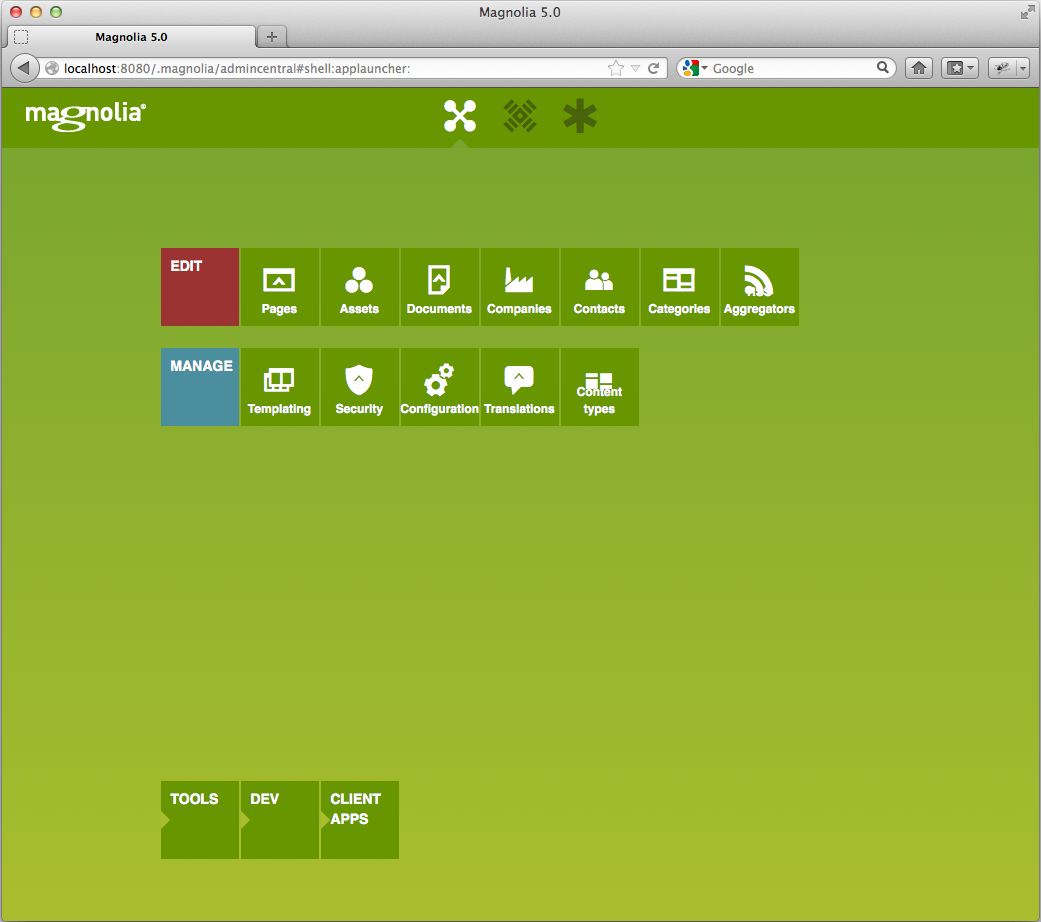
\includegraphics[width=\textwidth]{magnolia_shell.png}
	\caption{Magnolia Shell}
	\label{fig:m_shell}
\end{figure}

From the user interface point of view MagnoliaShell conceptually resembles the
browser viewport \cite{mshell_wiki}.
Actually, it contains two viewports (\texttt{ ShellViewport}): one for the apps
and one - for the shell apps.
 The \emph{ application framework } utilizes the viewports as containers in
 \texttt{AppController} and \texttt{ShellAppController} implementation.

\emph{Locations framework} is also connected with MagnoliaShell. The latter acts
as a buffer between client and server sides in fragment handling process. The
client-side implementation of MagnoliaShell subscribes to GWT's History API
events, based on a fragment it resolves which type of an app it has to launch
and instructs the server accordingly. On the server-side the
\texttt{LocationHistoryHandler} de-serializes the received fragment into a
\texttt{Location} instance which is handled by either \texttt{AppController} or
\texttt{ShellAppController}: based on the location parameters the correct
sub-app is launched. The other way around - an app is able to initiate a
navigation event (e.g. when switching between two app due to some server side
logic), at the end simply forcing the browser to update its fragment silently
(without sending an event to subscribers).

\section{Actions}
http://wiki.magnolia-cms.com/display/DEV/Actions+API+and+configuration
http://wiki.magnolia-cms.com/display/MAGNOLIA5/UI+-+Actions
http://wiki.magnolia-cms.com/display/UX/The+action+bar+screens

\section{Dependency injection}
\input{include/architecture/di.tex}

\pagebreak
%\chapter{Project Implementation}
\label{implementation}
In Project Implementation chapter we will provide some specific details of the
system was built. We will touch the data binding problem, the gesture
recognition solution and some approaches to increase the client-side
performance. In addition to that we will give an example of a Magnolia 5.0 App
built on top of the aforementioned APIs.

\section{Server Side}

\section{Dialogs and Forms}
\input{include/architecture/forms_and_dialogs.tex}

\subsection{Workbench}

\subsection{Managing Multiple Browser Tabs With Vaadin 6}

\subsection{Wiring JCR with Vaadin Container API}
 
\subsection{JcrNodeAdapter}

\subsection{AbstractJcrContainer}

\subsection{Server Push}

\subsubsection{Principles of IcePush component}

\subsubsection{Application of IcePush in MagnoliaShell}

\section{Client Side}

\subsection{Fast Transitions with JQueryWrapper and CSS3 Delegate Plugin}

\subsubsection{Plugin Architecture Examination}

\subsubsection{Implementation}

\subsection{Adding Touch Devices Support with MGWT Library. Gesture Recognition}

\subsubsection{Why use mgwt?}

\subsubsection{Conflicts between mgwt and Vaadin}

\subsubsection{SwipeHandler implementation}

\subsection{Vaadin. Developing Custom Vaadin Widgets Using RPC Interfaces and MVP}

\subsubsection{Importance of clear component implementation and fine-grained communication.}

\subsubsection{Widget RPC architecture and application in project}

\subsubsection{Example of appslauncher}

\subsection{Apps}

\subsection{Developing Magnolia 5.0 App Module}

\subsection{Messages App via Server Push Mechanism}

\subsection{Workbench and Pages Editor}

\section{Testing Server Side with JUnit and Mockito}

\pagebreak
%\section {Possibilities with Vaadin 7}
The upcoming release of Vaadin 7 could bring various improvements to the project such as:
\begin{itemize}
	\item Shared state/RPC for client-server communication.
	\item Faster client side implementation. 
	\item Easier integration of JavaScript libraries.
\end{itemize}
\pagebreak
%\section{Summary}
\pagebreak
%\begin{thebibliography}{9}

\bibitem{book_of_magnolia}
\emph{Book of Magnolia}
TODO: Add a Magnolia Book reference

\bibitem{Magnolia documentation}
  \emph{Magnolia documentation:} 
  
  http://documentation.magnolia-cms.com/index.html
  
\bibitem{node2bean}
  \emph{Node2Bean}

   %http://documentation.magnolia-cms.com/reference/configuration.html#Content2Bean

\bibitem{magnolia_customers}
  \emph{Magnolia customers:}
  
  http://www.magnolia-cms.com/clients/case-studies.html

\bibitem{poor_cms_experience}
  \emph{Poor CMS Experience}
  
  http://www.v3.co.uk/v3-uk/news/2012231/users-frustrated-poor-cms-functionality
  
\bibitem{cms_growth}
  \emph{The most popular 5 CMS:} 
  
  http://www.qarea.com/articles/most-popular-5-cms-choose-best-one-creation-your-Web Site

\bibitem{xpath}
  \emph{XPath}
  http://ru.wikipedia.org/wiki/XPath

\bibitem{drdobbs_cms_decouple}
  \emph{Magnolia Decouples the CMS for Developers:} 
  
  http://www.drdobbs.com/mobile/magnolia-decouples-the-cms-for-developer/240006760  
 
 \bibitem{BorisCraft}
  \emph{Raising the Bar in CMS Usability with Vaadin:} 
  
  http://www.betterfasterbigger.com/2011/02/raising-bar-in-cms-usability-with.html
  
 \bibitem{ArchitectureManifests}
  \emph{Magnolia CMS 5.0 - Architecture manifests:} 
  
  http://philipp-baerfuss-magnolia.blogspot.ch/2011/03/magnolia-50-architecture-manifests.html
  
 \bibitem{magnolia_shell}
  \emph{MagnoliaShell} 
  
  http://wiki.magnolia-cms.com/display/DOCS/Magnolia+Shell
 
 \bibitem{dlipp_why_vaadin}
  \emph{Why to use Vaadin in Magnolia 5.0?} 
   
  http://www.slideshare.net/DanielLipp/mgnl5whyvaadin
 \bibitem{why_vaadin_philipp}
 \emph{Why Vaadin - line of argument:}
  http://philipp-baerfuss-magnolia.blogspot.ch/2010/08/why-vaadin-line-of-argument.html
  
 \bibitem{BoV} 
  \emph{Book of Vaadin:}
  
  https://vaadin.com/book/-/page/preface.html
  
 \bibitem{GWT}{GWT}
  \emph{GWT:}
  
  https://developers.google.com/web-toolkit/overview
  
 \bibitem{ux_andreas}
 \emph{How Magnolia 5 avoids CMS UX pitfalls:}
 http://ma-ui.blogspot.fi/search?updated-max=2012-08-15T16:02:00%2B02:00&max-results=7&reverse-paginate=true
 
 \bibitem{cms_decomposition}
 \emph{CMS Decomposition:}
 http://www.betterfasterbigger.com/2013/01/cms-deconstructed-is-user-experience.html
 
 \bibitem{mobile_first}
 \emph{Why Magnolia 5 is mobile first}
 http://www.betterfasterbigger.com/2012/09/why-magnolia-5-is-mobile-first.html
 
 \bibitem{bkg_of_new_design}
 \emph{Magnolia 5.0 and the needs of today's seekers of user experience simplicity}
 http://ma-ui.blogspot.fi/2012/06/byod-or-how-magnolia-5-will-also-boost.html
 
 \bibitem{virtual_presence}
 \emph{Virtual Presence Management}
 http://www.magnolia-cms.com/dms/products/tech-briefs/vpm/Magnolia-Tech-Brief-VPM.pdf
 
 \bibitem{def_bind}
 \emph{Deferred Binding in GWT:}
 https://developers.google.com/web-toolkit/doc/latest/DevGuideCodingBasicsDeferred

\bibitem{gwt_memory_leaks}
 \emph{DOM Events, Memory Leaks and you:} 
 http://tinyurl.com/d84p57v 
  
\bibitem{jsni}
\emph{JSNI:}
https://developers.google.com/web-toolkit/doc/latest/DevGuideCodingBasicsJSNI?hl=ru

\bibitem{jquery}
\emph{JQuery:}
http://tinyurl.com/28bngz

\bibitem{gwt_historian}
\emph{GWT History API:}
https://developers.google.com/web-toolkit/doc/latest/DevGuideCodingBasicsHistory

\bibitem{activities_places}
https://developers.google.com/web-toolkit/doc/latest/DevGuideMvpActivitiesAndPlaces

\bibitem{why_apps_in_m5}
http://ma-ui.blogspot.fi/2012/09/apps-make-your-own-custom-ui.html

\bibitem{mshell_wiki}
http://wiki.magnolia-cms.com/display/DOCS/Magnolia+Shell

\bibitem{maui_apps}
http://ma-ui.blogspot.ru/2012/09/apps-make-your-own-custom-ui.html

\bibitem{wiki_app_framework}
http://wiki.magnolia-cms.com/display/DOCS/App+Framework

\bibitem{google_guice}
\emph{Google Guice}
https://code.google.com/p/google-guice/
\end{thebibliography}

% insert references
\bibliographystyle{unsrt}
%\bibliography{your bibliography's file name}

% make sure pagecount is correct even if references overflow to a new page
\pagebreak\addtocounter{page}{-1}
\eofpages
\appendices

% create your appendix chapters with command \appchapter{some name} instead
% of \chapter{some name} for the automagic page counting to work

%\input{file name of appchapter xxx}

\eofapppages
\end{document}